\documentclass[10pt,onecolumn,letterpaper]{article}
%% Welcome to Overleaf!
%% If this is your first time using LaTeX, it might be worth going through this brief presentation:
%% https://www.overleaf.com/latex/learn/free-online-introduction-to-latex-part-1

%% Researchers have been using LaTeX for decades to typeset their papers, producing beautiful, crisp documents in the process. By learning LaTeX, you are effectively following in their footsteps, and learning a highly valuable skill!

%% The \usepackage commands below can be thought of as analogous to importing libraries into Python, for instance. We've pre-formatted this for you, so you can skip right ahead to the title below.

%% Language and font encodings
\usepackage[spanish,english]{babel}
\usepackage[utf8x]{inputenc}
\usepackage[T1]{fontenc}

%% Sets page size and margins
\usepackage[a4paper,top=3cm,bottom=2cm,left=3cm,right=3cm,marginparwidth=1.75cm]{geometry}

%% Useful packages
\usepackage{amsmath}
\usepackage{graphicx}
\usepackage[colorinlistoftodos]{todonotes}
\usepackage[colorlinks=true, allcolors=blue]{hyperref}

%% Title
\title{
		%\vspace{-1in} 	
		\usefont{OT1}{bch}{b}{n}
		\normalfont \normalsize \textsc{MIE 1624 Introduction to Data Science and Analytics} \\ [10pt]
		\huge Assignment 1: Salary Analysis Report \\
}

\usepackage{authblk}

\author{Yunjie Xu 1008601951}


	\affil{\small{Department of Mechanical and Industrial Engineering, University of Toronto}}


\begin{document}
\maketitle

\selectlanguage{english}


%%\begin{abstract}
%%The abstract is probably what you'll be writing last, and should be roughly 300 words in length. Your abstract will get published whether or not your team wins the challenge, so make sure to do an extra good job of it! An easy way to structure your abstract is to write individual summaries of the four parts of your paper (Introduction, Methods, Results, Discussion) and then put them together once you're done.
%%\end{abstract} \\ 
%%\\ 
%%{\textbf{Keywords} \\
%%pick, 3-5, good, keywords}

\section*{Introduction}
This assignment aims to explore the nature of women's representation in data science field. Q25 "What is your current yearly compensation?" is the target column in this assignment.

\section*{Question 1}
I integrated those whose gender is not “Man” or “Woman” into “Gender Minority”. I found that woman only accounted for 16.13\% of people who working in data science field, while man constituted 82.14\%. In general,
Country(Figure 1), Age(Figure 2), Education(Figure 3), and Professional Experience(Figure 4) are all very important factors in influencing salary.In Gender, Men usually have higher salary than women with the same education level(Figure 5, Figure 6) or experience(Figure 7, Figure 8) or age(Figure 9, Figure 10). In education, people with higher degree are more easy to get higher salary generally. In experience and age, people with long experience usually can get higher rewards as well as the olders usually can earn more.

\section*{Question 2}
\subsection*{a}
The second part focuses on estimating the difference between men's average and women's(Figure 11). I observe that the mean salary for men is higher than women as well as median,and other quartiles, while men's salary fluctuate more than women's salary. I also plotted box plot of salary separately(Figure 12, Figure 13), I observed outliers.

\subsection*{b}
According to the p-value from the T-test result is much smaller than 0.05 threshold from the code, thus reject the null hypothesis should be rejected. So, I may conclude that the difference of mean salaries of men and women is statistically significant. However,since two data samples are not normally distributed based on that both two histograms do not show like a bell shape (Figure 14). So the normality assumptions are violated. Thus, this conclusion may not be reliable and T-test is not suitable here.

\subsection*{c}
I used random.sample function of Python to bootstrap the samples with sample sizes of men and women being relative to their sizes. After replicated 1000 times, it is found that the bootstrapped means are very close to the actual mean salaries of men and women. The two distributions, men and women’s bootstrapped mean salary, have clear different means with a small overlap. It further proved our findings of higher salary for men previously(Figure 15). And Figure 16 shows the difference in means for men and women.

\subsection*{d}
 Both bootstrapped distribution distribute normally, the normality assumption can be satisfied in this time. The T-score is 98.14 and p-value of our t-test is statistically significant with $\alpha = 0.05$. I thus reject the null hypothesis that there is no difference between mean salary of men and women in the data science field, based on bootstrapped data. Thus I can conclude that the difference of mean salaries of men and women is statistically significant . 
 
\subsection*{e}
I found that the bootstrap is a method of doing inference in a way that does not require assuming a parametric form for the population distribution. It means the method can fix the dataset which fails the normality test. In addition, there is a high statistically significant difference between mean salary of men and women in the data science field, while the mean difference based on bootstrapping is 16467.47. 

\section*{Question 3}
\subsection*{a}
I found that masters accounted the largest proportion of people in data science field, while the doctor accounted least. And I observe that the mean salary for doctor is higher than master and bachelor as well as median,and other quartiles, while doctor's salary fluctuate more(Figure 17). I also made box plot here(Figure 18, Figure 19, Figure 20). 


\subsection*{b}
ANOVA is not suitable here. There are three primary assumptions in ANOVA. Firstly, the responses for each factor level have a normal population distribution. Secondly, these distributions have the same variance. Thirdly, the data are independent. I plotted histograms like q2.b above (Figure 21), I found normality assumption failed. Then, I also calculated variances, I found equal variance assumption also failed. Though, the f-score is 109.76, thus the null hypothesis should be rejected. I conclude there is at least one group mean is different than others.

\subsection*{c}
Similarly, using random.sample to bootstrap the samples with sample sizes of three groups being relative to their sizes. It is found that the bootstrapped means are very close to the actual means and among three groups, doctoral displays a higher variance(Figure 22).  Figure 23, 24, 25 demonstrate the bootstrapped differences among the pairs within three groups. On average, mean salary for doctorates is \$18268.67 higher than masters , while the mean salary for masters is \$17123.06 higher than bachelors. 

\subsection*{d}
ANOVA is still not suitable here.Because all bootstrapped distribution distribute normally, the normality assumption can be satisfied after bootstrapping. But from doctoral displays a higher variance(Figure 22), thus equal variance assumption is still violated. Though, the f-score is 10938.95, larger than q3.b. So, the null hypothesis still be rejected. I conclude there is at least one group mean is different than others.

\subsection*{e}
In future, I can use bootstrapping method do inference without assuming a parametric form for the population distribution. It is very useful when normality assumption is need but violate. However, bootstrapping method can only fix distributions to normal distribution with different variance, thus this method cannot help with fixing equal variance assumption.

\section*{Appendix}

\appendix
\begin{figure}[htbp]
  \centering
  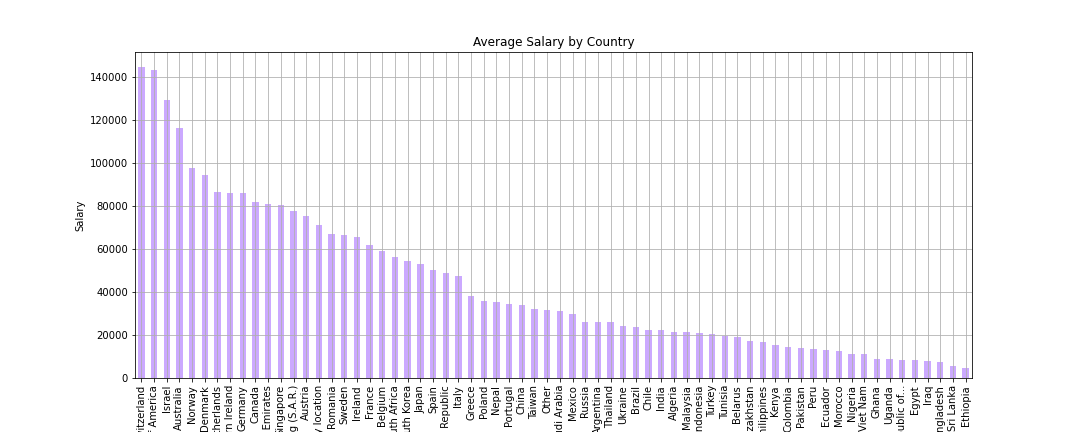
\includegraphics[width=1\textwidth]{f1.png}
  \caption{Average Salary by Country}
\end{figure}

\begin{figure}[htbp]
  \centering
  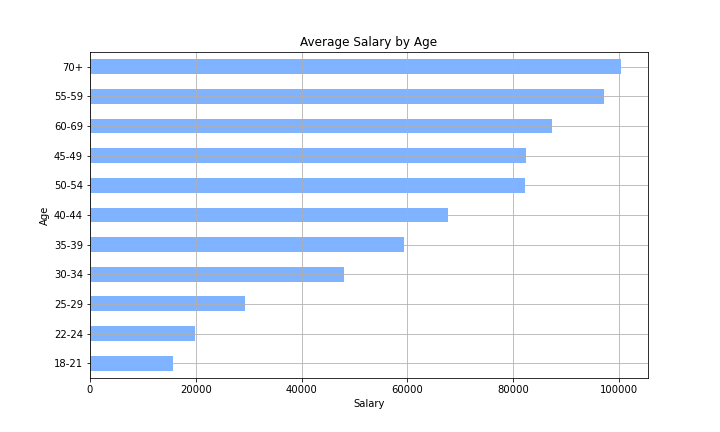
\includegraphics[width=1\textwidth]{f2.png}
  \caption{Average Salary by Age}
\end{figure}

\begin{figure}[htbp]
  \centering
  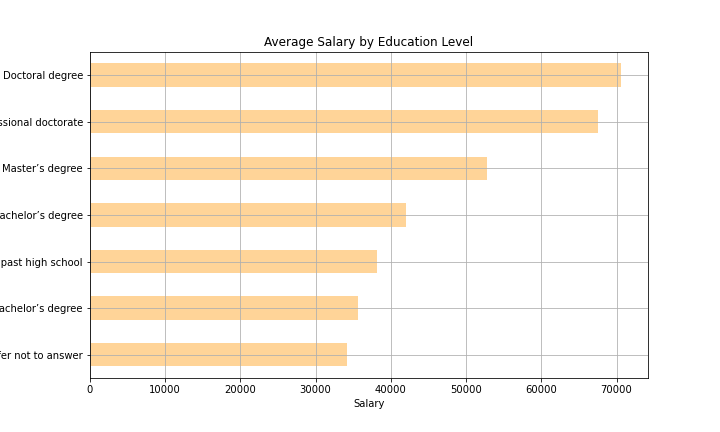
\includegraphics[width=1\textwidth]{f3.png}
  \caption{Average Salary by Education}
\end{figure}

\begin{figure}[htbp]
  \centering
  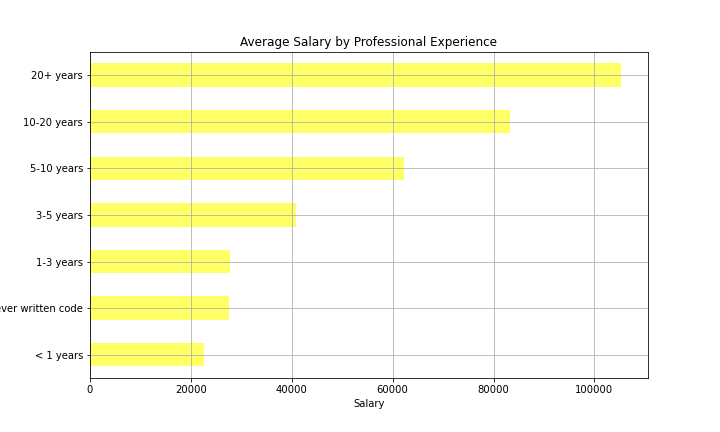
\includegraphics[width=1\textwidth]{f4.png}
  \caption{Average Salary by Experience}
\end{figure}

\begin{figure}[htbp]
  \centering
  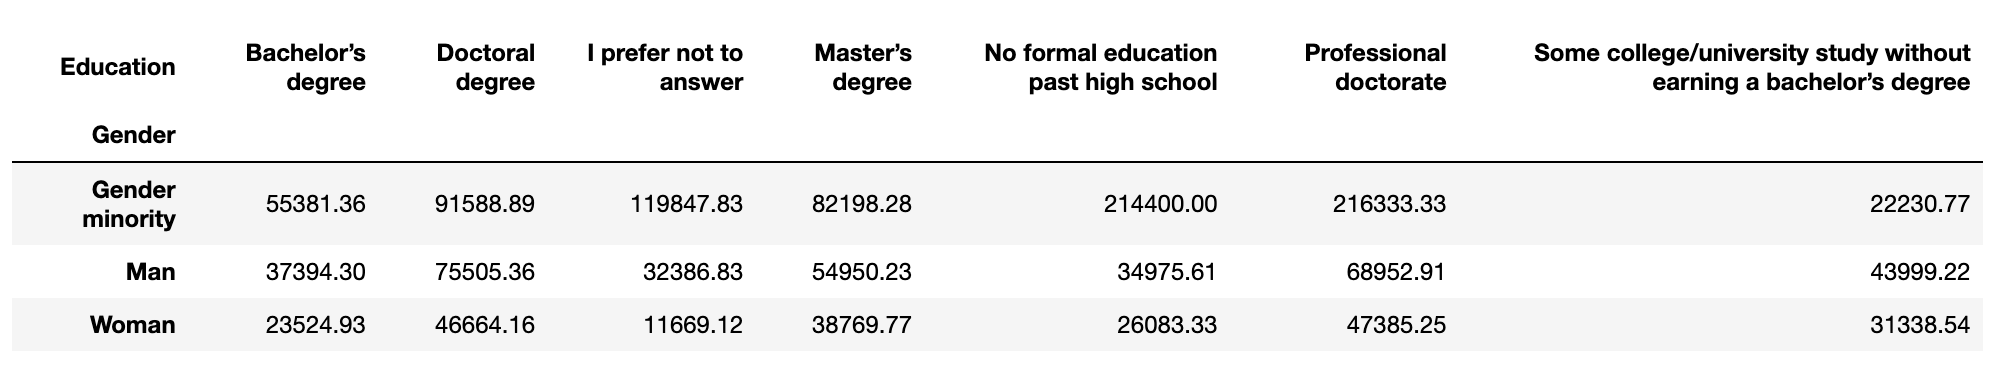
\includegraphics[width=1\textwidth]{f5.png}
  \caption{Table of Salary Based on Different Gender and Education Level}
\end{figure}

\begin{figure}[htbp]
  \centering
  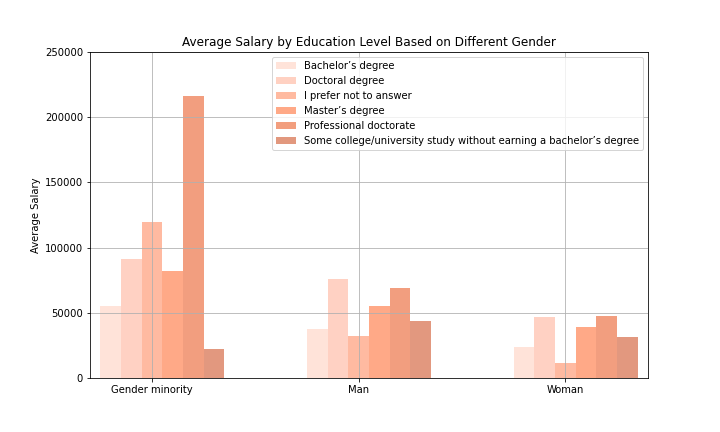
\includegraphics[width=1\textwidth]{f6.png}
  \caption{Plot of Salary Based on Different Gender and Education Level}
\end{figure}

\begin{figure}[htbp]
  \centering
  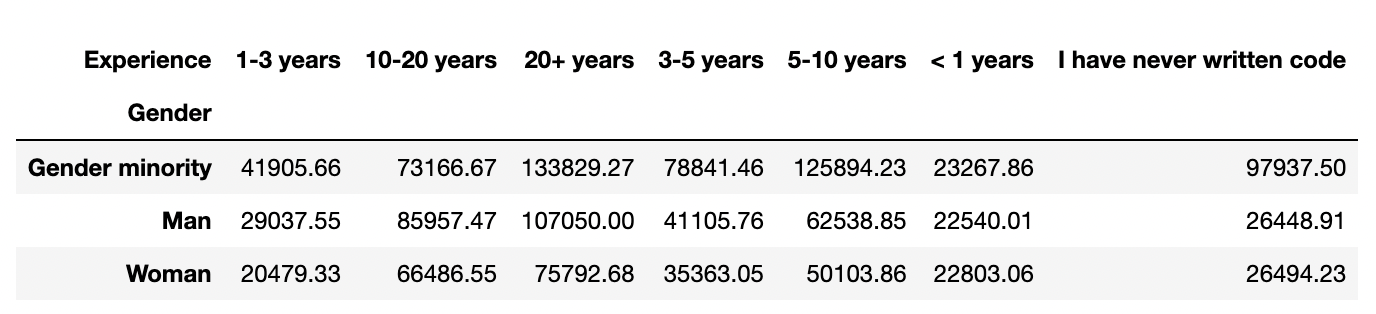
\includegraphics[width=1\textwidth]{f7.png}
  \caption{Table of Salary Based on Different Gender and Experience}
\end{figure}

\begin{figure}[htbp]
  \centering
  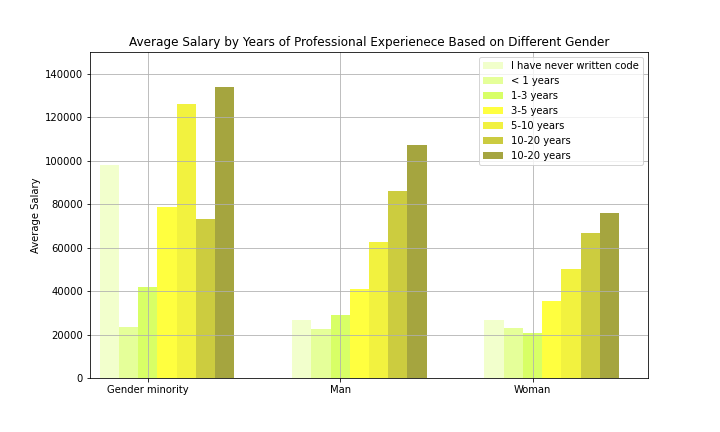
\includegraphics[width=1\textwidth]{f8.png}
  \caption{Plot of Salary Based on Different Gender and Experience}
\end{figure}

\begin{figure}[htbp]
  \centering
  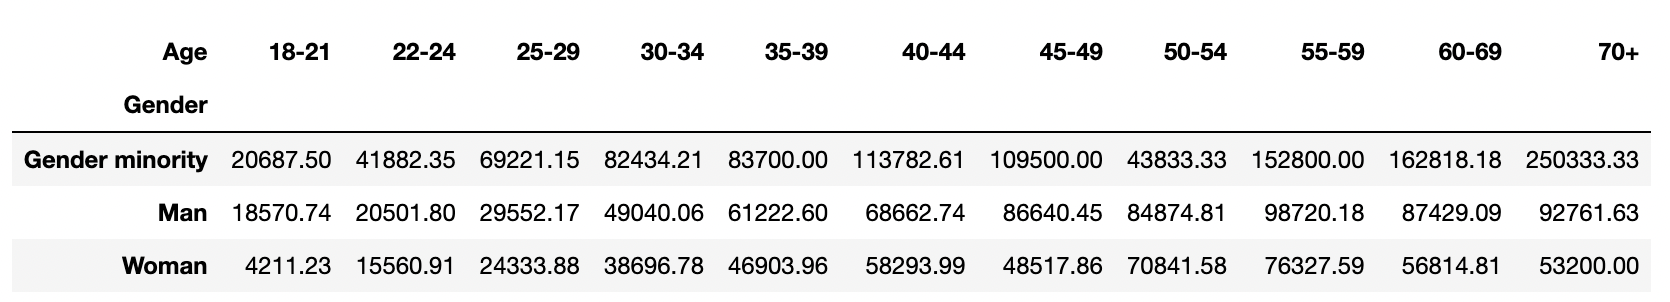
\includegraphics[width=1\textwidth]{f9.png}
  \caption{Table of Salary Based on Different Gender and Age}
\end{figure}

\begin{figure}[htbp]
  \centering
  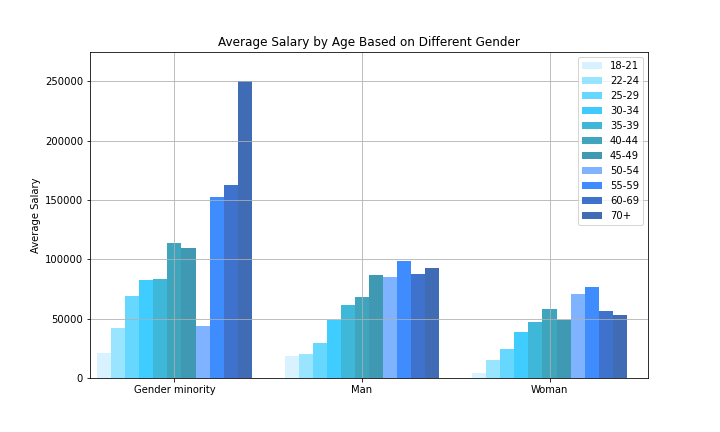
\includegraphics[width=1\textwidth]{f10.png}
  \caption{Plot of Salary Based on Different Gender and Age}
\end{figure}

\begin{figure}[htbp]
  \centering
  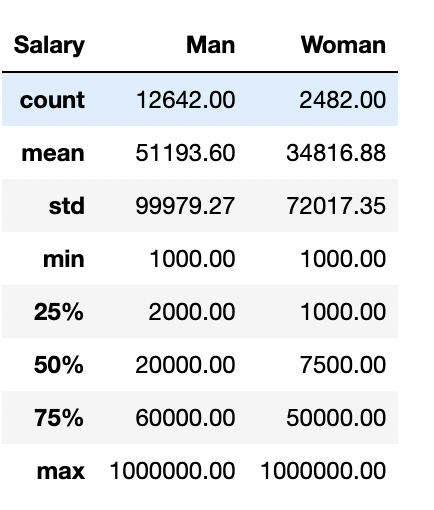
\includegraphics[width=0.5\textwidth]{f11.png}
  \caption{Table of Salary Based Gender}
\end{figure}

\begin{figure}[htbp]
  \centering
  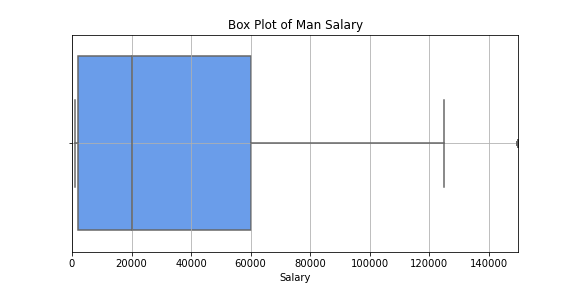
\includegraphics[width=0.75\textwidth]{f12.png}
  \caption{Box Plot of Men's Salary}
\end{figure}

\begin{figure}[htbp]
  \centering
  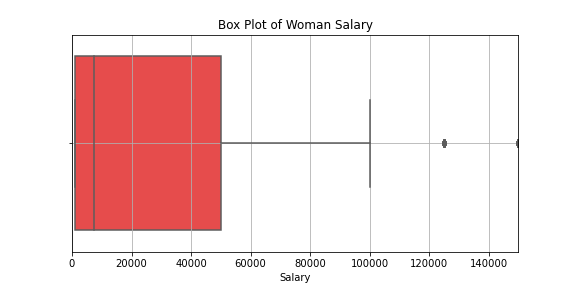
\includegraphics[width=0.75\textwidth]{f13.png}
  \caption{Box Plot of Women's Salary}
\end{figure}

\begin{figure}[htbp]
  \centering
  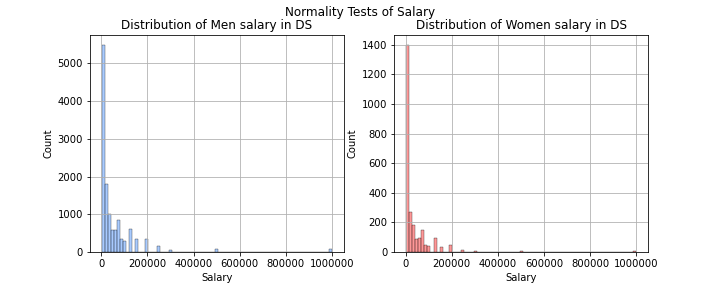
\includegraphics[width=1\textwidth]{f14.png}
  \caption{Normality Checking}
\end{figure}

\begin{figure}[htbp]
  \centering
  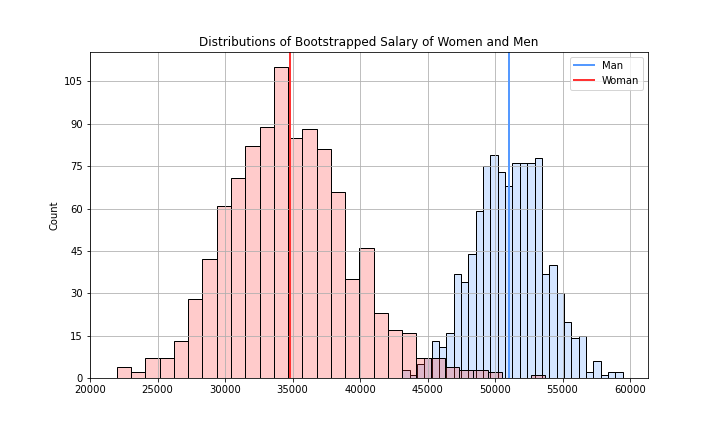
\includegraphics[width=1\textwidth]{f15.png}
  \caption{Distributions of Bootstrapped Salary of Women and Men}
\end{figure}

\begin{figure}[htbp]
  \centering
  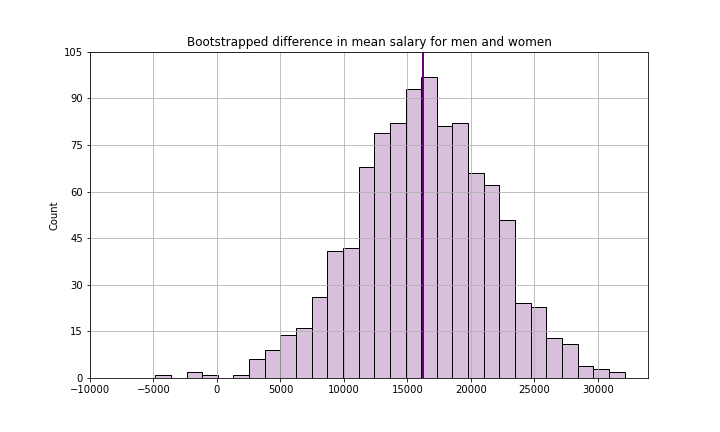
\includegraphics[width=1\textwidth]{f16.png}
  \caption{Bootstrapped difference in mean salary for men and women}
\end{figure}

\begin{figure}[htbp]
  \centering
  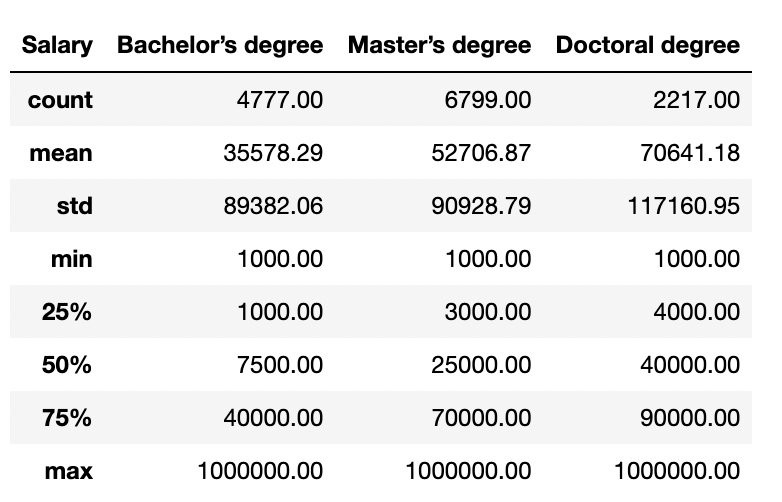
\includegraphics[width=0.75\textwidth]{f17.png}
  \caption{Table of Salary Based Degree}
\end{figure}

\begin{figure}[htbp]
  \centering
  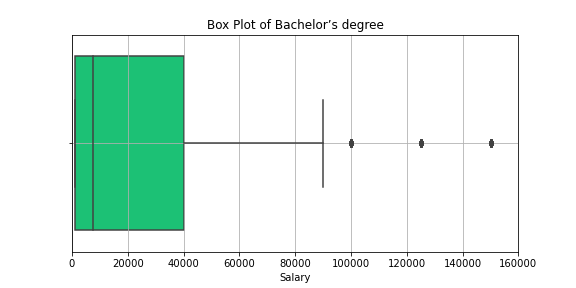
\includegraphics[width=.75\textwidth]{f18.png}
  \caption{Box Plot of Bachelor’s degree}
\end{figure}

\begin{figure}[htbp]
  \centering
  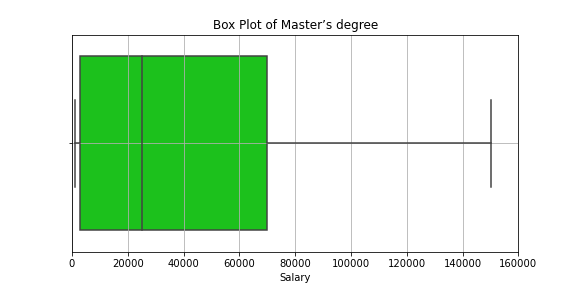
\includegraphics[width=.75\textwidth]{f19.png}
  \caption{Box Plot of Master’s degree}
\end{figure}

\begin{figure}[htbp]
  \centering
  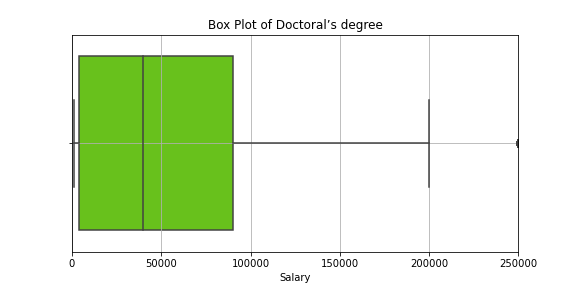
\includegraphics[width=.75\textwidth]{f20.png}
  \caption{Box Plot of Doctor’s degree}
\end{figure}

\begin{figure}[htbp]
  \centering
  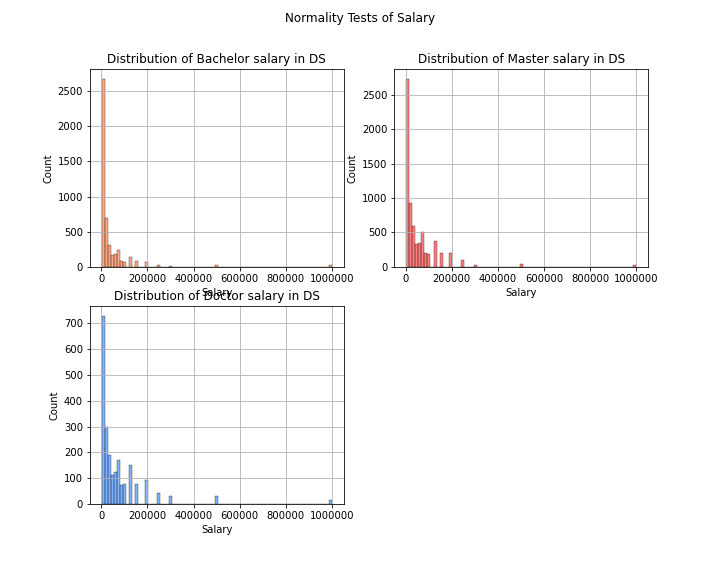
\includegraphics[width=1\textwidth]{f21.png}
  \caption{Assumption Checking for Q3}
\end{figure}

\begin{figure}[htbp]
  \centering
  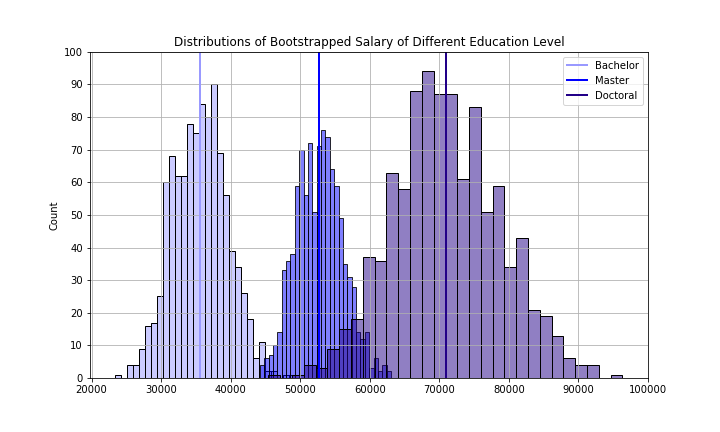
\includegraphics[width=1\textwidth]{f22.png}
  \caption{Distributions of Bootstrapped Salary of Different Education Level}
\end{figure}

\begin{figure}[htbp]
  \centering
  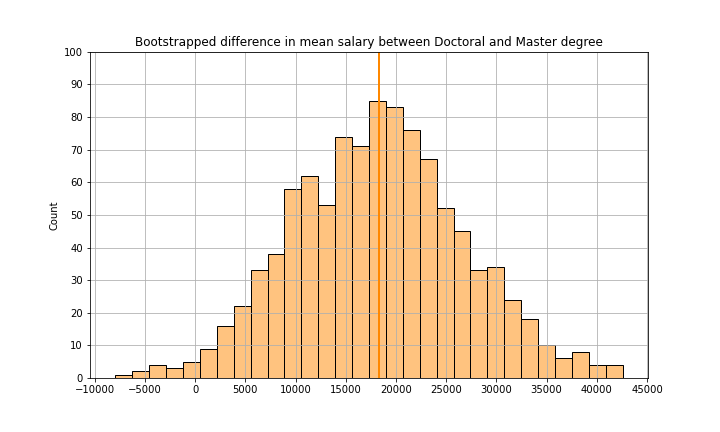
\includegraphics[width=1\textwidth]{f23.png}
  \caption{Bootstrapped difference in mean salary between Doctoral and Master degree}
\end{figure}

\begin{figure}[htbp]
  \centering
  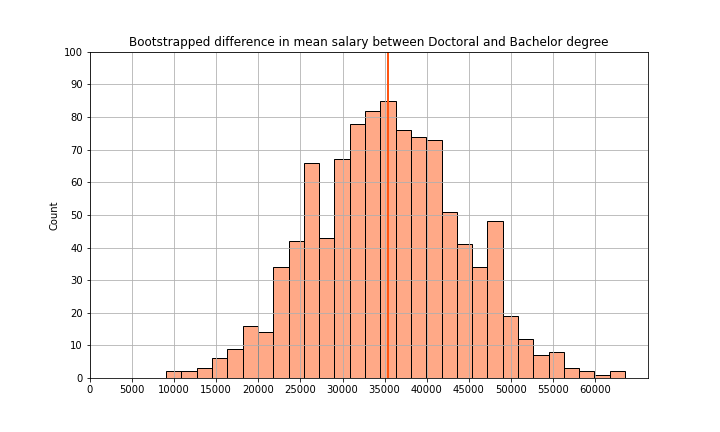
\includegraphics[width=1\textwidth]{f24.png}
  \caption{Bootstrapped difference in mean salary between Doctoral and Bachelor degree}
\end{figure}

\begin{figure}[htbp]
  \centering
  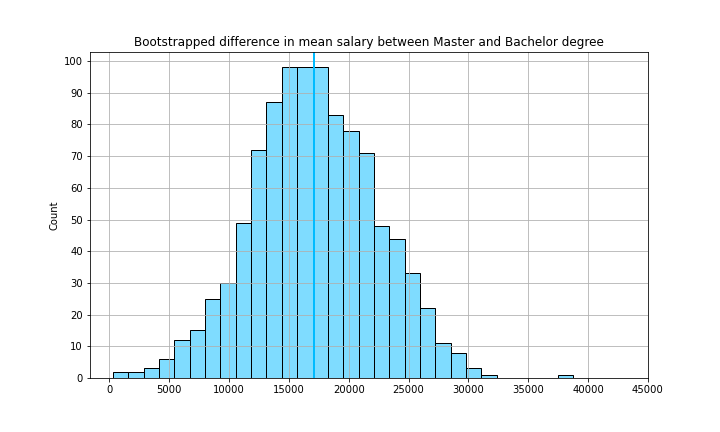
\includegraphics[width=1\textwidth]{f25.png}
  \caption{Bootstrapped difference in mean salary between Master and Bachelor degree}
\end{figure}

\end{document}